%!TEX root = ../Main.tex

%-------------------------------------------------------------------------------

\chapter{Clustering Methods}
Clustering refers to grouping data into different clusters or classes. We do this to get observations or samples clustered into groups where they share some similarities. This is used extensively in the field of machine learning. An example of clusters or classes could be handwritten numbers (0-9). Each number has distinct features which can be divided into clusters. An unsupervised problem would be to divide the numbers into subclasses. In a supervised problem we would already have made the clustering and then divide new samples into the already known clusters, or in other words, predict some outcome based on the sample.

\subsection{K-means clustering}
K-means clustering is a simple method of clustering data. It works by having a number (K) mean-vectors and assigning a sample to the mean-vector that it's closest to. On \cref{fig:k-means_clustering} 150 sample have been generated and three different values for K. It is easy to see that the K-means method tries to cluster samples that are close to each other in the same class.

\begin{figure}[H]
	\centering
	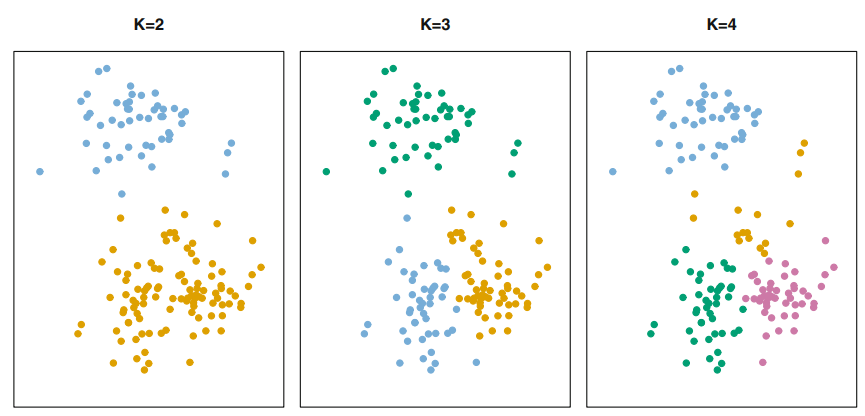
\includegraphics[width=12cm]{Img/K-means_clustering.PNG}
	\caption{K-means clustering example}
	\label{fig:k-means_clustering}
\end{figure} 

This works by minimizing the squared euclidean distance to each mean-vector. 

\begin{equation} \label{transformed_linear_regression_eq}
minimize_{C1...C_{K}}\{\sum_{k=1}^{K}\dfrac{1}{\lvert C_{k} \rvert} \sum_{i,i'\in C_{k}}^{} \sum_{j=1}^{p}(x_{ij}-x_{i'j})^{2} \}
\end{equation}

$\lvert C_{k}\rvert$ denotes the number of samples in the kth cluster. Or the within variation of the kth cluster which is the sum of all the pairwise squared euclidean distances between the observations in the kth cluster, divided by the total number of samples in kth cluster.

To implement this as an algorithm the book covers how this should be done. 

\begin{figure}[H]
	\centering
	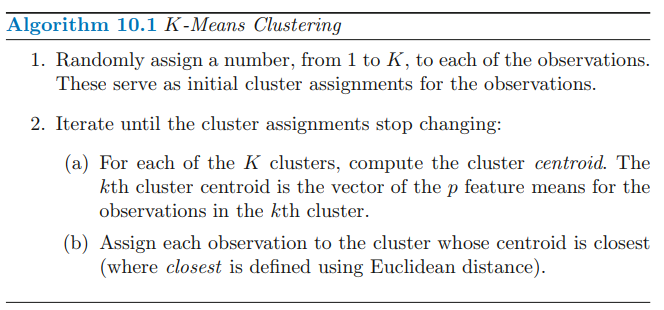
\includegraphics[width=12cm]{Img/Algo_kmeans.PNG}
	\caption{K-means clustering pseudo code}
	\label{fig:k-Algo_kmeans.PNG}
\end{figure} 

In action this algorithm performs well and can be seen on \cref{Algo_kmeans_inaction}

\begin{figure}[H]
	\centering
	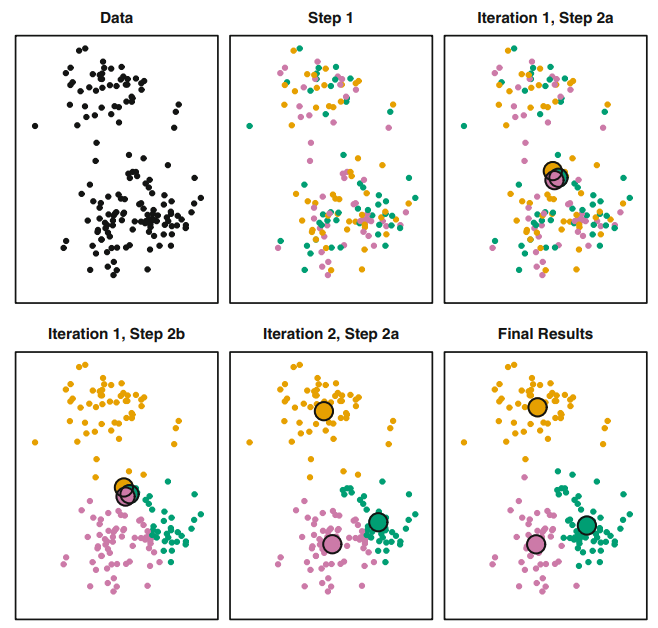
\includegraphics[width=10cm]{Img/Kmean_algo_example.PNG}
	\caption{K-means clustering in action}
	\label{fig:k-Algo_kmeans_inaction.PNG}
\end{figure} 


\subsection{Hierarchical Clustering}
